\documentclass[noinfoline]{imsart}


\usepackage{bm}
\usepackage{graphics,epsfig,rotate,lscape,graphicx,amsmath,amsthm,amssymb,float,amsfonts,amsbsy,hyperref,delarray,sectsty,amsfonts,amscd,pifont}
\usepackage{color,multirow}
\usepackage{algorithmicx}
\usepackage{algorithm}
\usepackage{enumerate}
\usepackage{microtype}
\usepackage{wrapfig}

\usepackage{geometry}
\geometry{letterpaper,left=1.2in,right=1.2in,top=1.2in,bottom=1.1in}

\bibliographystyle{plain}


\newtheorem{claim}{Claim}
\newtheorem{proposition}{Proposition}
\newtheorem{theorem}{Theorem}
\newtheorem{lemma}{Lemma}
\newtheorem{conjecture}{Conjecture}
\newtheorem{corollary}[theorem]{Corollary}
\newtheorem{definition}{Definition}
\newtheorem{notation}{Notation}
\renewcommand{\labelenumi}{(\roman{enumi})}
\newcommand{\bx}{\boldsymbol x}
\newcommand{\by}{\boldsymbol y}
\newcommand{\bl}{\boldsymbol l}
\newcommand{\bk}{\boldsymbol k}
\newcommand{\re}{\text{\,\rm re}}
\newcommand{\im}{\text{\,\rm im}}
\newcommand{\bs}{\boldsymbol}

\newcommand{\pinv}{\hat\phi}
\newcommand{\sinv}{\hat\psi}



% --------------------------------------
\begin{document}



\begin{frontmatter}
\title{BayesLenseSPTpol}
\runtitle{BayesLenseSPTpol}

\begin{abstract}
At this point there is nothing in here but a few derivations.
\end{abstract}

% \begin{keyword}
% \kwd{CMB}
% \kwd{gravitational lensing}
% \kwd{Bayesian}
% \kwd{Gibbs sampler}
% \kwd{Polarization}
% \end{keyword}

\end{frontmatter}


Here is the general polarization lensing setup which includes both a gravitational potential and a rotational potential.
\begin{align*}
\widetilde Q(x) &\equiv  Q(x+\nabla \phi(x)+\nabla^\perp \psi(x)) \\
\widetilde U(x) &\equiv  U(x+\nabla \phi(x)+\nabla^\perp \psi(x))
\end{align*}
where $Q, U$ denote the unlensed CMB polarization fields, $\phi$ denotes the lensing potential, $\psi$ denotes a field rotation potential and $\nabla^\perp \equiv(\frac{\partial}{\partial x_2}, -\frac{\partial}{\partial x_1})$.
We observe $\widetilde Q, \widetilde U$ and try to estimate $\phi$, $\psi$, $Q$ and $U$.


\section{Old stuff:}
Here is a plot of the power spectrums I was using for the simulations
\begin{center}
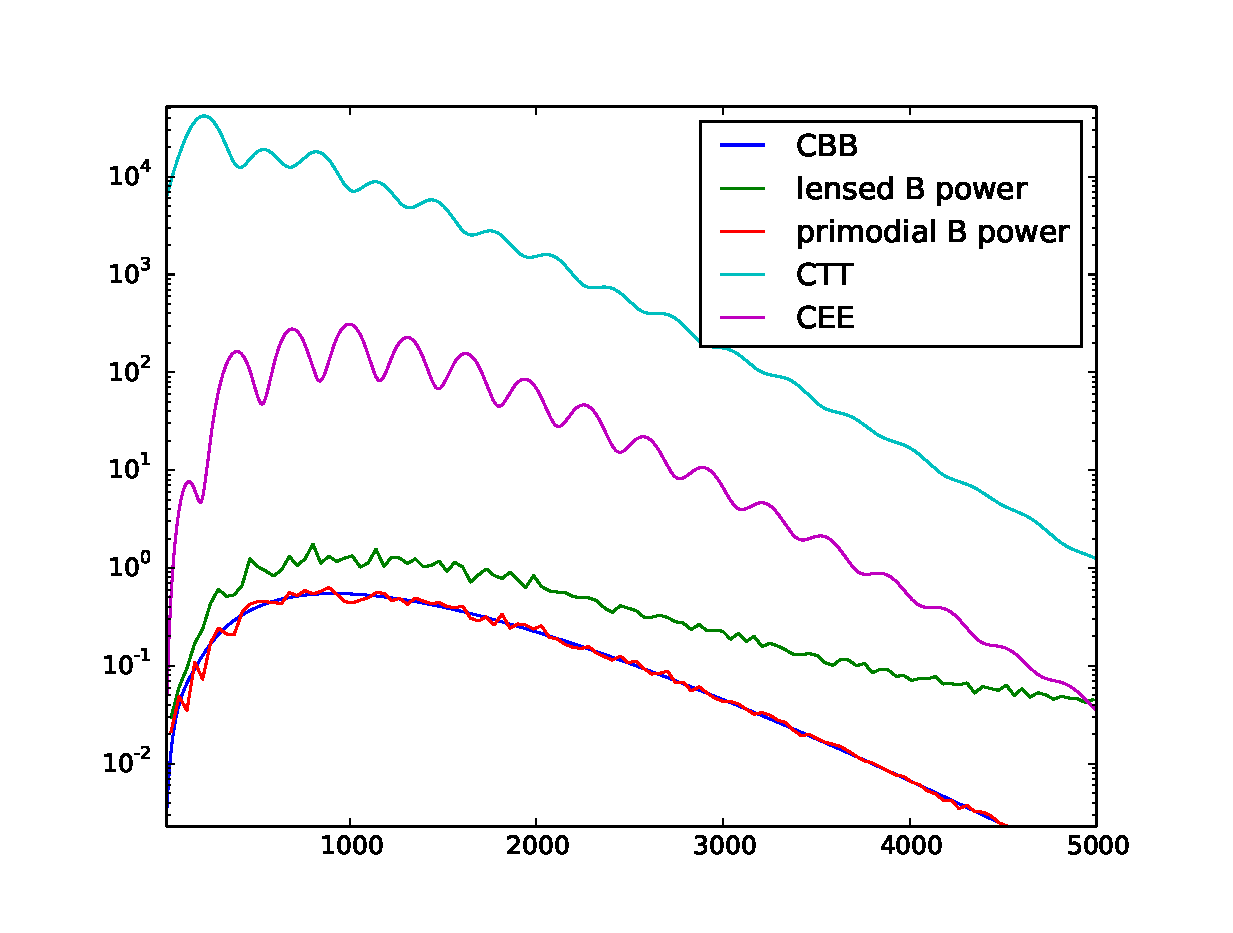
\includegraphics[height = 2.2in]{spectrum1.eps}%
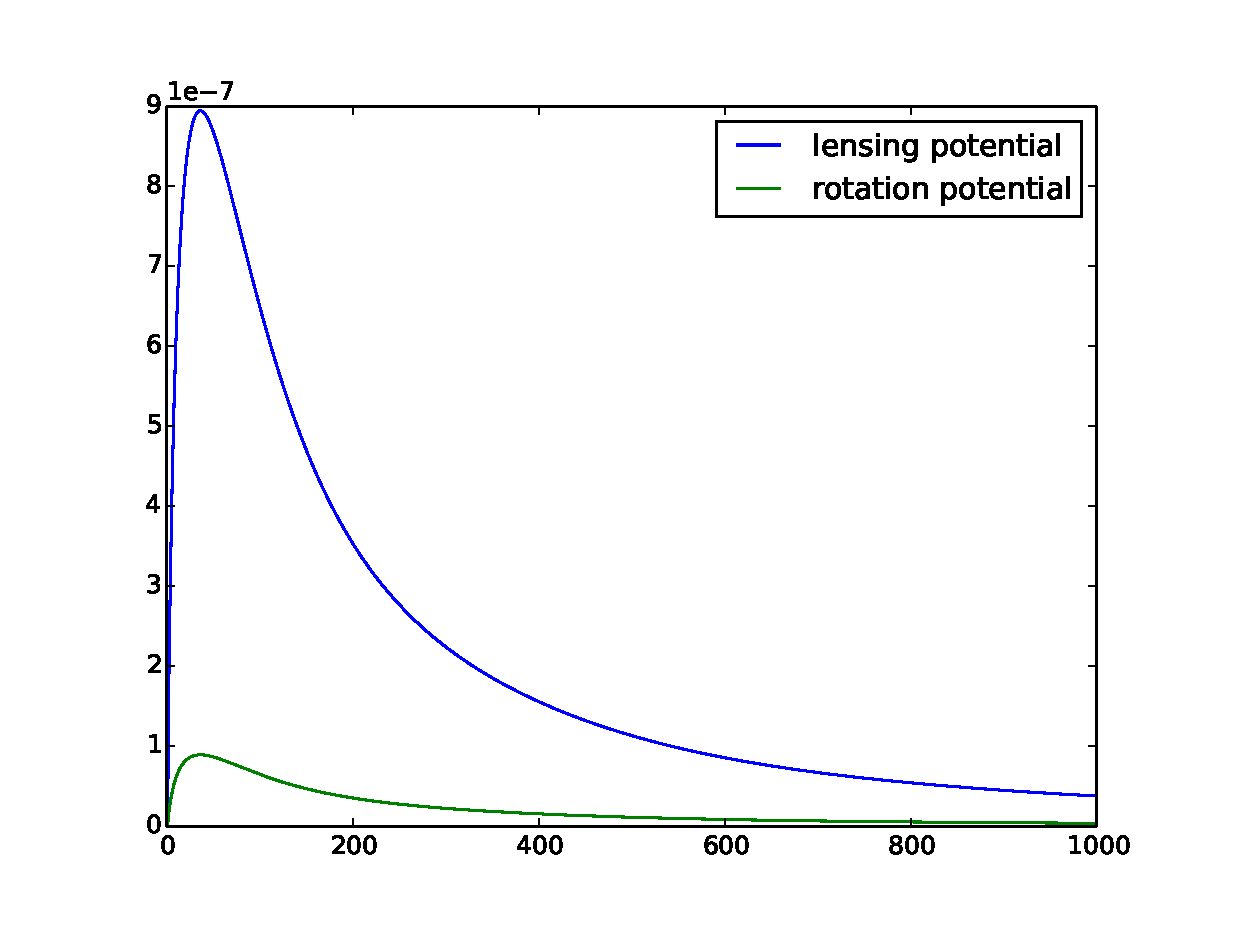
\includegraphics[height = 2.2in]{spectrum2.eps}
\end{center}
\newpage
Here is a plot of the maximum likelihood estimate of $\phi$ and $\psi$ from $\tilde Q, \tilde U$
\begin{center}
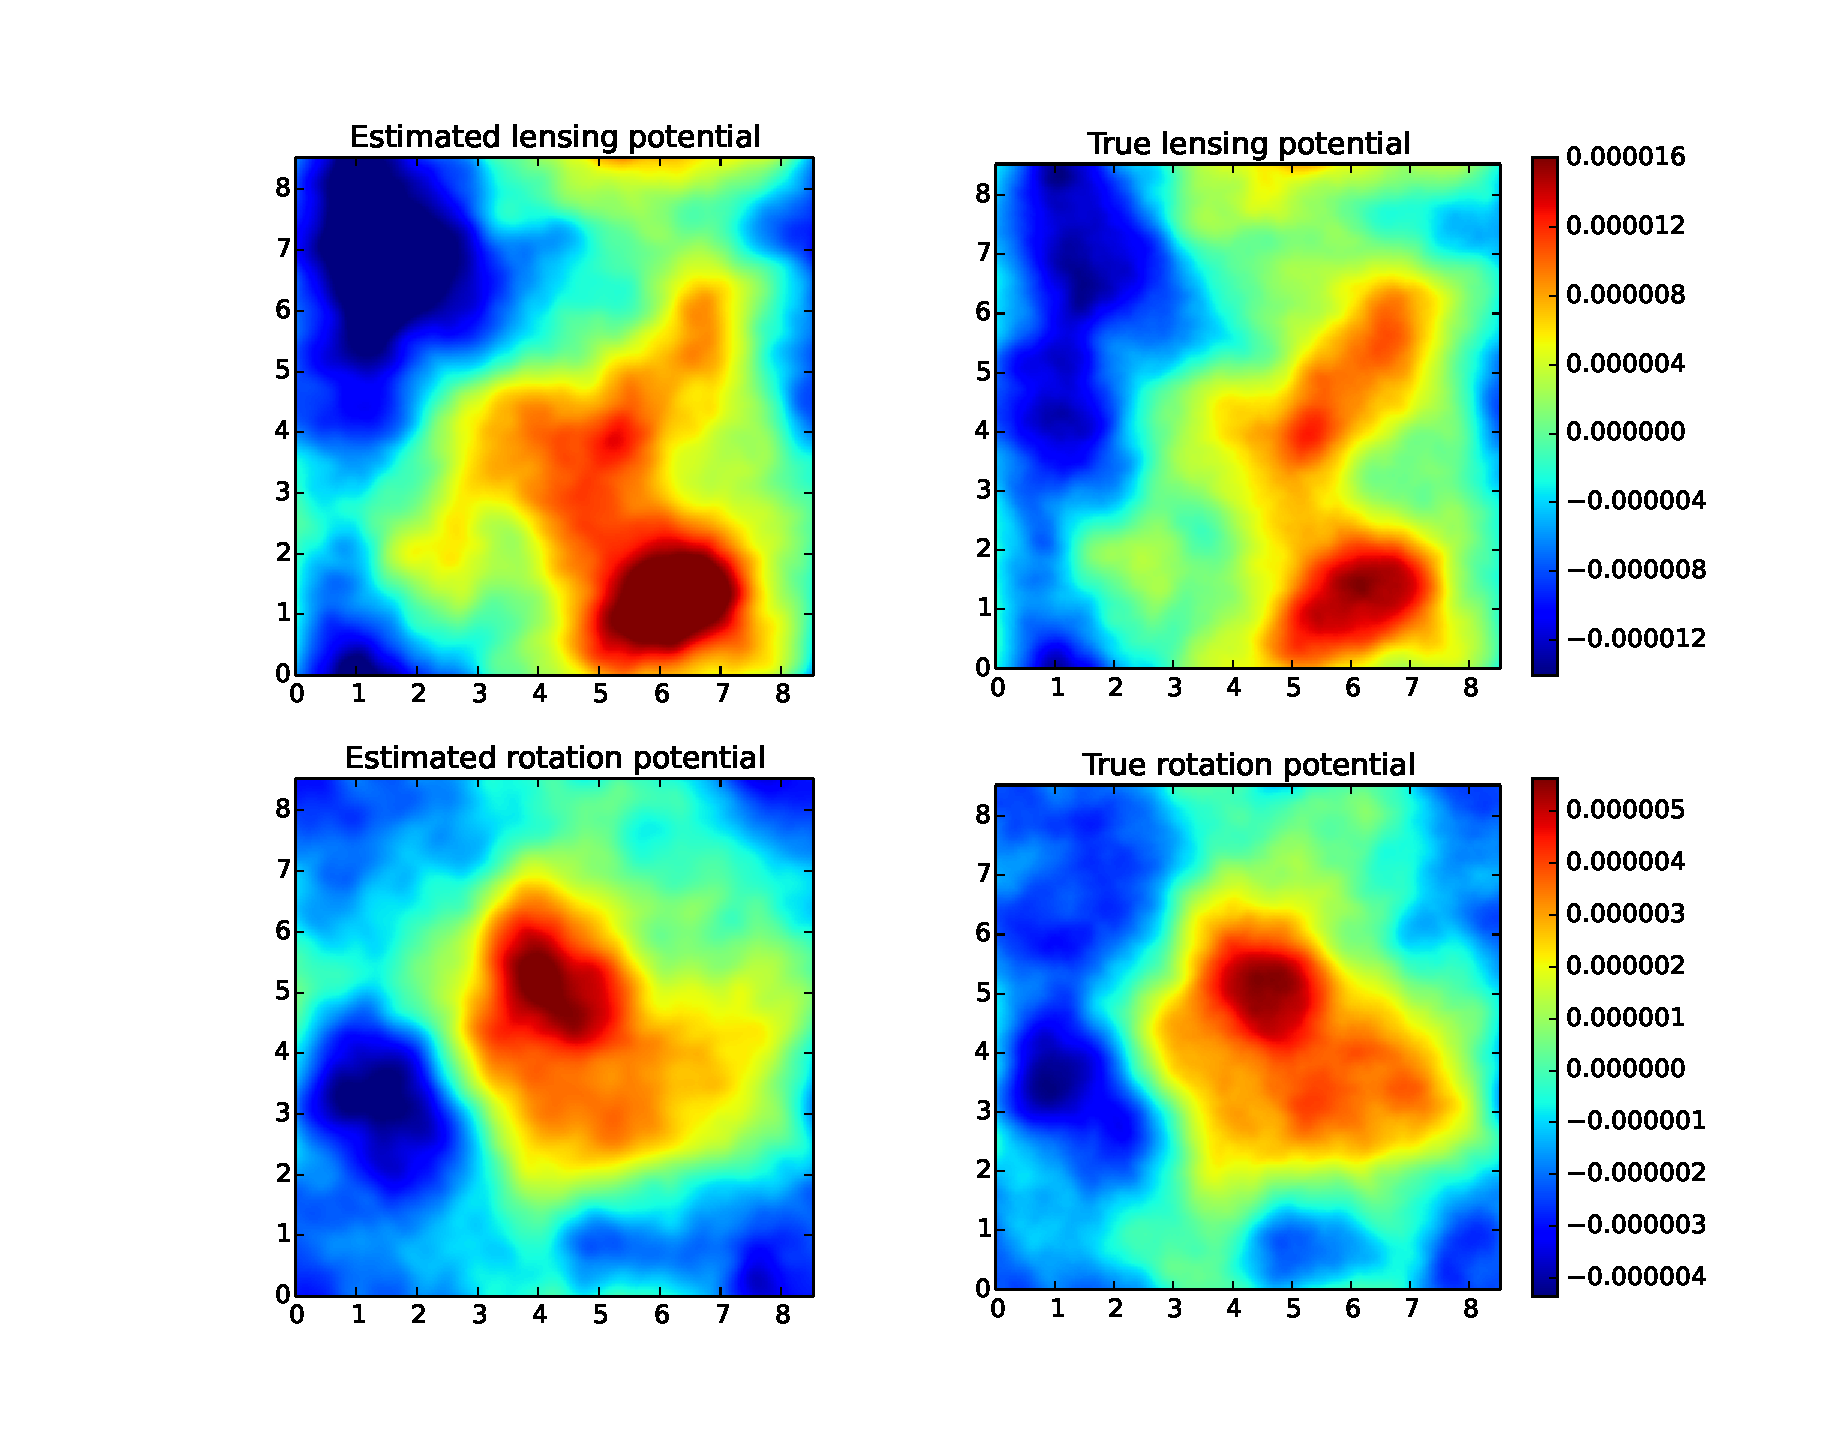
\includegraphics[height = 5.2in]{images.eps}
\end{center}
Finally, here is a plot of the power of the estimated unlensed primodial $B$ mode. In particular I use the estimates $\hat \phi$ and $\hat \psi$ and unlense the observed $\tilde Q, \tilde U$.
\begin{center}
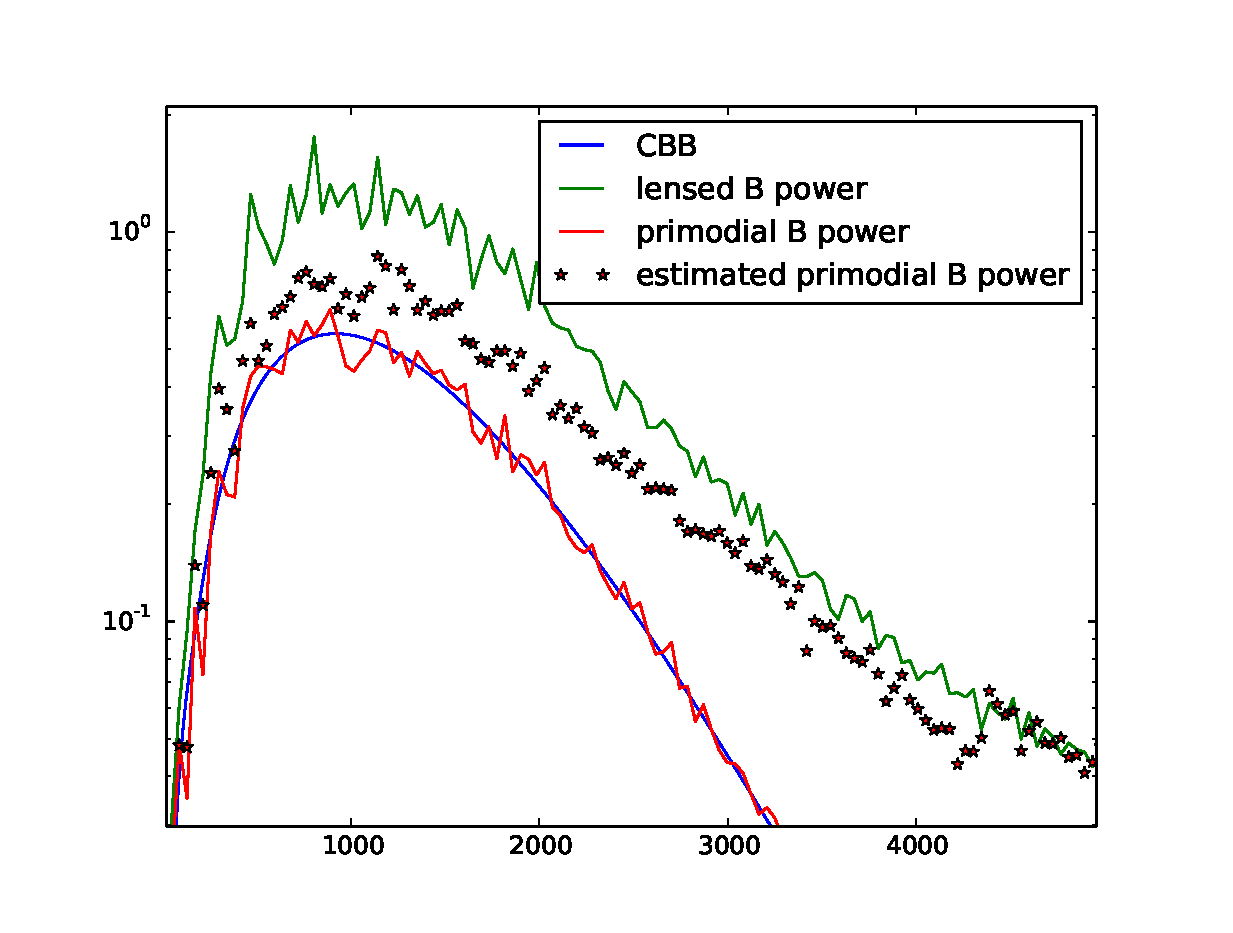
\includegraphics[height = 2.5in]{spectrum3.eps}
\end{center}


%%%%%%%%%%%%%%%%%%%%
%
%  appendix
%
%%%%%%%%%%%%%%%%%%%%%%
\appendix

\section{}




If we exclude the zero frequency $l = 0$ we get
\begin{align*}
-\log P( \widetilde Q,  \widetilde U| \phi,\psi) - c_1
&=  \frac{1}{2}\int_{\Bbb R^2}\left[ \frac{\bigl| \widetilde E_k^{\phi\psi}\bigr|^2}{C_k^{EE}}   +  \frac{\bigl| \widetilde B_k^{\phi\psi}\bigr|^2}{C_k^{BB}} \right]dk  \\
&=  \frac{1}{2}\int_{\Bbb R^2}\left[ \frac{\bigl|-\cos(2\varphi_k) \widetilde Q_k^{\phi\psi} -\sin(2\varphi_k) \widetilde U_k^{\phi\psi} \bigr|^2}{C_k^{EE}}   + \frac{\bigl|\sin(2\varphi_k) \widetilde Q_k^{\phi\psi} -\cos(2\varphi_k) \widetilde U_k^{\phi\psi} \bigr|^2}{C_k^{BB}} \right]dk   \\
&=  \frac{1}{2}\int_{\Bbb R^2} \left[\frac{\cos^2(2\varphi_k)}{C_k^{EE}} +\frac{\sin^2(2\varphi_k)}{C_k^{BB}} \right]| \widetilde Q_k^{\phi\psi}|^2   dk\\
&\qquad + \frac{1}{2}\int_{\Bbb R^2}  \left[\frac{\cos^2(2\varphi_k)}{C_k^{BB}} +\frac{\sin^2(2\varphi_k)}{C_k^{EE}}\right] | \widetilde  U_k^{\phi\psi}|^2 dk\\
&\qquad\quad + \frac{1}{2}\int_{\Bbb R^2}\left[ \frac{2\sin(2\varphi_k)\cos(2\varphi_k)(C_k^{BB} - C_k^{EE})}{C_k^{EE} C_k^{BB}}\right] \widetilde  Q_k^{\phi\psi} ( \widetilde U_k^{\phi\psi})^*  dk
\end{align*}
where $c_1$ is a  constant,  $ Y^{\phi\psi}(x)\equiv  Y(x-\nabla \phi(x)-\nabla^\perp \psi(x))$ and $\nabla^\perp \equiv(\frac{\partial}{\partial x_2}, -\frac{\partial}{\partial x_1})$. Notice that in the last term in the above display, I've implicity used the fact that
\[ \int_{\Bbb R^2}M_k \widetilde  Q_k^{\phi\psi} ( \widetilde U_k^{\phi\psi})^*  dk = \int_{\Bbb R^2}M_k ( \widetilde Q_k^{\phi\psi})^* \widetilde  U_k^{\phi\psi}  dk  \]
whenever $M_{k} = M_{-k}$.


\begin{claim} Let $M_{k}$ real and symmetric in $k$. Let $X(x)$ and $Y(x)$ be real fields. Define $X^{\phi\psi}(x)\equiv X(x - \nabla \phi(x) - \nabla^\perp \psi(x))$ and similarly for $Y^{\phi\psi}$. Then
\begin{align*}
&\frac{\partial}{\partial \phi_l}  \int_{\Bbb R^2}   X^{\phi\psi}_k (Y^{\phi\psi}_k)^* M_kdk =
\phantom{-}il_q 2dk \int_{\Bbb R^2}\Bigl( [(\nabla^q X)^{\phi\psi}]_{k+l} {Y^{\phi\psi}_k}^* \,\,\,\,\,\,+ [(\nabla^q Y)^{\phi\psi}]_{k+l} {X^{\phi\psi}_k}^*\Bigr) M_k \frac{dk}{2\pi} \\
&\frac{\partial}{\partial \psi_l}  \int_{\Bbb R^2}   X^{\phi\psi}_k (Y^{\phi\psi}_k)^* M_kdk =
-il_q {2dk} \int_{\Bbb R^2}\Bigl( [(\nabla^{\perp,q} X)^{\phi\psi}]_{k+l} {Y^{\phi\psi}_k}^* + [(\nabla^{\perp,q} Y)^{\phi\psi}]_{k+l} {X^{\phi\psi}_k}^*\Bigr) M_k\frac{dk}{2\pi}
\end{align*}
\end{claim}




%%%%%%%%%%%%%%% lemma
\begin{lemma}
\label{partialconj}
\begin{align}
\frac{\partial  X^{\phi\psi}_k}{\partial \phi_{ l} }  &=  \phantom{-}il_q[(\nabla^q X)^{\phi\psi}]_{k+l}\frac{dk}{\pi}&
\frac{\partial  X^{\phi\psi}_k}{\partial \phi^*_{ l} } &=  -il_q [(\nabla^q X)^{\phi\psi}]_{k-l}\frac{dk}{\pi} \\
\frac{\partial  X^{\phi\psi}_k}{\partial \psi_{ l} }  &=  -il_q[(\nabla^{\perp,q} X)^{\phi\psi}]_{k+l}\frac{dk}{\pi}&
\frac{\partial  X^{\phi\psi}_k}{\partial \psi^*_{ l} } &=  \phantom{-}il_q [(\nabla^{\perp,q} X)^{\phi\psi}]_{k-l}\frac{dk}{\pi}.
\end{align}
where $\nabla^q  X\equiv \frac{\partial  X}{\partial x_q}$.
\end{lemma}
\begin{proof}
First notice
\begin{align}
\label{partial1}
\frac{\partial}{\partial \re \phi_{ l}} \nabla^q \phi(x)  &= \int_{\Bbb R^2} i  k_q e^{ix \cdot k} \frac{\partial \phi_k}{\partial \re \phi_l }  \frac{d k}{2\pi}
=\left[i  l_q e^{ix \cdot  l}  - i  l_q e^{-i x \cdot  l}  \right] \frac{d k}{2\pi}   \\
\label{partial2}
\frac{\partial}{\partial \im \phi_{ l}}\nabla^q \phi(x) &= \int_{\Bbb R^2} i  k_q e^{ix \cdot  k} \frac{\partial \phi_ k}{\partial \im \phi_{l} }  \frac{d k}{2\pi}
=\left[-  l_q e^{ix \cdot  l}  -  l_q e^{-i x \cdot  l}  \right] \frac{d k}{2\pi}.
\end{align}
Therefore
\begin{align}
\frac{\partial}{\partial \phi_{l}}\nabla^q \phi(x)  &=  - i  l_q e^{-i x \cdot l} \frac{dk}{\pi}   \\
\frac{\partial}{\partial \phi^*_{ l}}\nabla^q \phi(x) &= \phantom{-} il_q e^{ix \cdot  l}\frac{dk}{\pi}.
\end{align}
This implies
\begin{align}
\nonumber \frac{\partial X^{\phi\psi}_k}{\partial \phi_{ l} }
&=  \frac{\partial}{\partial  \phi_{ l} } \int_{\Bbb R^2}  e^{-ix \cdot k} X(x-\nabla \phi(x)-\nabla^\perp \psi(x))\frac{dx}{2\pi} \\
\nonumber &= \sum_{q=1,2}  \int_{\Bbb R^2} e^{-ix \cdot k} \nabla^q X(x-\nabla \phi(x)-\nabla^\perp\psi(x))\left[ -\frac{\partial}{\partial \phi_{l}}\nabla^q \phi(x)\right]\frac{dx}{2\pi}\\
\nonumber &= \sum_{q=1,2}  \int_{\Bbb R^2} e^{-ix \cdot k} \left[(\nabla^q X)^{\phi\psi}(x)\right]\left[  i  l_q e^{-i x \cdot l} \frac{dk}{\pi}\right]\frac{dx}{2\pi}
\end{align}
Similarly
\begin{align}
\frac{\partial X^{\phi\psi}_k }{\partial \phi^*_l }
&= \sum_{q=1,2}  \int_{\Bbb R^2} e^{-ix \cdot k} \left[(\nabla^q X)^{\phi\psi}(x)\right]\left[  -i  l_q e^{i x \cdot l}\frac{dk}{\pi} \right]\frac{dx}{2\pi}.
\end{align}
Conversely
\begin{align}
\nonumber \frac{\partial X^{\phi\psi}_k}{\partial \psi_{ l} }
&=  \frac{\partial}{\partial  \psi_{ l} } \int_{\Bbb R^2}  e^{-ix \cdot k} X(x-\nabla \phi(x)-\nabla^\perp \psi(x))\frac{dx}{2\pi} \\
\nonumber &=  \int_{\Bbb R^2} e^{-ix \cdot k} \nabla^1 X(x-\nabla \phi(x)-\nabla^\perp\psi(x))\left[- \frac{\partial}{\partial \psi_{l}}\frac{\partial\psi(x)}{\partial x_2}\right]\frac{dx}{2\pi}\\
 &\phantom{=}  +\int_{\Bbb R^2} e^{-ix \cdot k} \nabla^2 X(x-\nabla \phi(x)-\nabla^\perp\psi(x))\left[ \frac{\partial}{\partial \psi_{l}}\frac{\partial\psi(x)}{\partial x_1}\right]\frac{dx}{2\pi}\\
 \nonumber &=  \int_{\Bbb R^2} e^{-ix \cdot k} \nabla^1 X(x-\nabla \phi(x)-\nabla^\perp\psi(x))\left[ i  l_2 e^{-i x \cdot l} \frac{dk}{\pi}\right]\frac{dx}{2\pi}\\
 &\phantom{=}  +\int_{\Bbb R^2} e^{-ix \cdot k} \nabla^2 X(x-\nabla \phi(x)-\nabla^\perp\psi(x))\left[-  i  l_1 e^{-i x \cdot l} \frac{dk}{\pi}\right]\frac{dx}{2\pi} \\
 \nonumber &= \sum_{q=1,2}  \int_{\Bbb R^2} e^{-ix \cdot k} \left[(\nabla^{\perp,q} X)^{\phi\psi}(x)\right]\left[ - i  l_q e^{-i x \cdot l} \frac{dk}{\pi}\right]\frac{dx}{2\pi}
\end{align}
since $\nabla^{\perp,1}=\nabla^2$ and $\nabla^{\perp,2}=-\nabla^1$. Similary
\begin{align}
\nonumber \frac{\partial X^{\phi\psi}_k}{\partial \psi^*_{ l} }
&=  \frac{\partial}{\partial  \psi_{ l} } \int_{\Bbb R^2}  e^{-ix \cdot k} X(x-\nabla \phi(x)-\nabla^\perp \psi(x))\frac{dx}{2\pi} \\
\nonumber &=  \int_{\Bbb R^2} e^{-ix \cdot k} \nabla^1 X(x-\nabla \phi(x)-\nabla^\perp\psi(x))\left[- \frac{\partial}{\partial \psi^*_{l}}\frac{\partial\psi(x)}{\partial x_2}\right]\frac{dx}{2\pi}\\
 &\phantom{=}  +\int_{\Bbb R^2} e^{-ix \cdot k} \nabla^2 X(x-\nabla \phi(x)-\nabla^\perp\psi(x))\left[ \frac{\partial}{\partial \psi^*_{l}}\frac{\partial\psi(x)}{\partial x_1}\right]\frac{dx}{2\pi}\\
 \nonumber &=  \int_{\Bbb R^2} e^{-ix \cdot k} \nabla^1 X(x-\nabla \phi(x)-\nabla^\perp\psi(x))\left[ -i  l_2 e^{i x \cdot l}\frac{dk}{\pi} \right]\frac{dx}{2\pi}\\
 &\phantom{=}  +\int_{\Bbb R^2} e^{-ix \cdot k} \nabla^2 X(x-\nabla \phi(x)-\nabla^\perp\psi(x))\left[  i  l_1 e^{i x \cdot l}\frac{dk}{\pi} \right]\frac{dx}{2\pi} \\
 \nonumber &= \sum_{q=1,2}  \int_{\Bbb R^2} e^{-ix \cdot k} \left[(\nabla^{\perp,q} X)^{\phi\psi}(x)\right]\left[  i  l_q e^{i x \cdot l} \frac{dk}{\pi}\right]\frac{dx}{2\pi}
\end{align}
\end{proof}





%%%%%%%%%%%% lemma
\begin{lemma}
\label{forreal}
If $A(x)$ and $B(x)$ are real scalar fields then  the two  integrals,  $\int_{\Bbb R^2} i\bigl\{ A_{k-l}  -   A_{k+l}  \bigr\} B^*_k dk$ and  $\int_{\Bbb R^2}\bigl\{  A_{k-l}  +    A_{k+l}   \bigr\} B^*_k dk$, are both real numbers.
\end{lemma}


\begin{proof}
By a simple change of variables it is clear that
$\int_{\Bbb R^2} \left(i\bigl\{ A_{k-l}  -   A_{k+l}  \bigr\} B^*_k\right)^* dk = \int_{\Bbb R^2} i\bigl\{ A_{k^\prime-l} - A_{k^\prime+l}  \bigr\} B_{k^\prime}^* dk^\prime$ and $\int_{\Bbb R^2} \left(\bigl\{  A_{k-l}  +    A_{k+l}   \bigr\} B^*_k \right)^* dk  = \int_{\Bbb R^2} \bigl\{ A_{k^\prime-l} + A_{k^\prime+l}  \bigr\} B_{k^\prime}^* dk^\prime$.

% \begin{align*}
% \int_{\Bbb R^2} \left(i\bigl\{ A_{k-l}  -   A_{k+l}  \bigr\} B^*_k\right)^* dk &= \int_{\Bbb R^2} -i\bigl\{ A_{-k+l}  -   A_{-k-l}  \bigr\} B_{k} dk \\
% &= \int_{\Bbb R^2} -i\bigl\{ A_{k^\prime+l}  -   A_{k^\prime-l}  \bigr\} B_{-k^\prime} dk^\prime \\
% &= \int_{\Bbb R^2} i\bigl\{ A_{k^\prime-l} - A_{k^\prime+l}  \bigr\} B_{k^\prime}^* dk^\prime
% \end{align*}

% \begin{align*}
% \int_{\Bbb R^2} \left(\bigl\{  A_{k-l}  +    A_{k+l}   \bigr\} B^*_k \right)^* dk &= \int_{\Bbb R^2} \bigl\{ A_{-k+l}  +   A_{-k-l}  \bigr\} B_{k} dk \\
% &= \int_{\Bbb R^2} \bigl\{ A_{k^\prime+l}  +   A_{k^\prime-l}  \bigr\} B_{-k^\prime} dk^\prime \\
% &= \int_{\Bbb R^2} \bigl\{ A_{k^\prime-l} + A_{k^\prime+l}  \bigr\} B_{k^\prime}^* dk^\prime
% \end{align*}
\end{proof}



%%%%%%%%%%%% lemma
The following lemma is equivalent to the so-called Convolution Theorem. We state it here for reference.
\begin{lemma}
\label{conv}
If $A(x)$ and $B(x)$ are real scalar fields then  $\int_{\Bbb R^2} A_{k+l}  B^*_k \frac{dk}{2\pi}= \int_{\Bbb R^2} e^{-ix\cdot l} A(x)B(x)\frac{dx}{2\pi}$.
\end{lemma}

% \begin{proof}
% \begin{align*}
% \int_{\Bbb R^2} A_{k+l}  B^*_k \frac{dk}{2\pi}
% & = \int_{\Bbb R^2} \int_{\Bbb R^2} e^{-x\cdot (k+l)} A(x) B_{k}^*  \frac{dx}{2\pi}   \frac{dk}{2\pi} \\
% & = \int_{\Bbb R^2}e^{-ix\cdot l} A(x) \left[\int_{\Bbb R^2} e^{-x\cdot k} B_{k}^*     \frac{dk}{2\pi}\right] \frac{dx}{2\pi}\\
% & = \int_{\Bbb R^2}e^{-ix\cdot l} A(x) \left[\int_{\Bbb R^2} e^{x\cdot k} B_{k}     \frac{dk}{2\pi}\right]^* \frac{dx}{2\pi}\\
% &= \int_{\Bbb R^2} e^{-ix\cdot l} A(x)B^*(x)\frac{dx}{2\pi}\\
% &= \int_{\Bbb R^2} e^{-ix\cdot l} A(x)B(x)\frac{dx}{2\pi},\quad\text{since $B(x)$ is real.}
% \end{align*}
% \end{proof}

\section{Determinant}

Eq.(4.9) of Lewis 2006
\begin{align}
\tilde T_\ell
&= T_\ell -\int \frac{d^2\ell'}{2\pi} \ell'\cdot(\ell-\ell')\phi_{\ell-\ell'} T_{\ell'}\\
& -\frac{1}{2}\int \frac{d^2\ell_1}{2\pi}\frac{d^2\ell_2}{2\pi} \ell_1\cdot(\ell_1+\ell_2-\ell)\ (\ell_1\cdot\ell_2)
T_{\ell_1}\  \phi_{\ell_2}\phi_{\ell-\ell_1-\ell_2} \nonumber
\end{align}

\begin{align}
\langle \phi_\ell \phi_{-\ell'} \rangle=\langle \phi_\ell \phi_{\ell'}^* \rangle = \delta(\ell-\ell') C_\ell
= \frac{\delta_{\ell,\ell'}}{dl} C_\ell
\end{align}

\begin{align}
A_{\ell k}\equiv\frac{\partial \tilde T_\ell}{\partial T_k}
=& \delta_{\ell,k} + \sum_{\ell'}\frac{dl}{2\pi} \ell'\cdot(\ell-\ell')\phi_{\ell-\ell'} \delta_{\ell',k}\\
& -\frac{1}{2}\sum_{\ell_1,\ell_2} \frac{dl}{2\pi}\frac{dl}{2\pi} \ell_1\cdot(\ell_1+\ell_2-\ell)\ (\ell_1\cdot\ell_2)
\delta_{\ell_1,k} \phi_{\ell_2}\phi_{\ell-\ell_1-\ell_2} \nonumber\\
=& \delta_{\ell,k} + \frac{dl}{2\pi} k\cdot(\ell-k) \phi_{\ell-k}
-\frac{1}{2}\frac{dl}{2\pi}\frac{dl}{2\pi} \sum_{\ell_2}  k\cdot(k+\ell_2-\ell)\ (k\cdot\ell_2)
\phi_{\ell_2}\phi_{\ell-k-\ell_2}
\end{align}

Keep $O(\phi)$ for off-diagnal terms and $O(\phi^2)$ for diagnal terms, and accurate to $O(\phi^2)$ for $\det (A)$

\begin{align}
A_{\ell k}
&= \delta_{\ell,k} \left(1-\frac{dl^2}{8\pi^2}\sum_{\ell_2}   (k\cdot\ell_2)^2
  \phi_{\ell_2}\phi_{-\ell_2} \right) + \frac{dl}{2\pi} k\cdot(\ell-k)\phi_{\ell-k}\\
\det A
&=1-\frac{dl^2}{8\pi^2}\sum_k\sum_{\ell_2}   (k\cdot\ell_2)^2 \phi_{\ell_2}\phi_{-\ell_2}
-\frac{1}{2} \frac{dl^2}{4\pi^2} \sum_\ell \sum_{k\neq\ell} k\cdot(\ell-k)\ \ell\cdot(k-\ell)\phi_{\ell-k}\phi_{k-\ell}\nonumber\\
&=1-\frac{dl^2}{8\pi^2}\sum_k\sum_{\ell_2}   (k\cdot\ell_2)^2 \phi_{\ell_2}\phi_{-\ell_2}
+\frac{dl^2}{8\pi^2} \sum_k \sum_{\ell'}  (k\cdot\ell')\ (k+\ell')\cdot\ell'\phi_{\ell'}\phi_{-\ell'}\nonumber\\
&=1+\frac{dl^2}{8\pi^2} \sum_k \sum_{\ell'} (k\cdot\ell') {\ell'}^2 \phi_{\ell'}\phi_{-\ell'} \nonumber\\
&=1
\end{align}

Note that $\frac{\partial}{\partial \phi_l}
\equiv \frac{\partial}{\partial{\rm re} \phi_l} +i\frac{\partial}{\partial{\rm Im} \phi_l} $, then
$\frac{\partial}{\partial \phi_i} \phi_{l} = 2 \delta_{i,-l}$

\section{$C_l^{\pinv\pinv}, C_l^{\pinv\sinv}, C_l^{\sinv\sinv}$ and $C_l^{\phi\phi}$}

Using $f(x) = x + \nabla\phi(x)$,
$\nabla\pinv + \nabla^\perp \sinv = \nabla\phi(f^{-1}(x)) = \nabla\phi(x-\nabla\pinv-\nabla^\perp\sinv)$
and  $ f^{-1}(x)\simeq x -\nabla\phi(x) + (\nabla\phi\cdot\nabla)\nabla\phi,$
\begin{align}
  \nabla^2\pinv &= \nabla\cdot \left(\nabla\phi|_{x-\nabla\phi(x)+(\nabla\phi\cdot\nabla)\nabla\phi}\right)
\end{align}

\begin{align}
  \nabla^2\pinv
  &= \nabla\cdot \left(d|_{x-d+(d\cdot\nabla)d}\right)\nonumber\\
  &\simeq \nabla\cdot \left[d  - (d \cdot \nabla)d + [(d \cdot \nabla)d\cdot \nabla] d
  + \frac{1}{2}(d  \cdot \nabla)^2 d\right]\nonumber\\
  &=\nabla^2\phi - \partial_1(\vec d\cdot \nabla) d_1 - \partial_2(\vec d\cdot \nabla) d_2
  +\nabla\cdot [(d \cdot \nabla)d\cdot \nabla] d
  + \frac{1}{2}\partial_1(\vec d\cdot \nabla)^2d_1 + \frac{1}{2}\partial_2(\vec d\cdot \nabla)^2d_2
\end{align}


\begin{align}
  -l^2\pinv_l
  &= -l^2\phi_l - \int (k\cdot l)(k\cdot (k + l)) \phi_{k+l}\phi_k^*  \frac{d^2k}{2\pi}\nonumber\\
  & +\frac{1}{2}\int (m+k+l)\cdot k\  m\cdot k \ (k+2m)\cdot k\ \phi_{m+k+l}\phi_{m}^*\phi_{k}^*\frac{d^2k}{2\pi}\frac{d^2m}{2\pi}
\end{align}

\begin{align}
  l^4 C_l^{\pinv\pinv}
  &=l^4 C_l^{\phi\phi}  - l^2\int\frac{d^2k}{(2\pi)^2} (k\cdot l)(k^2+k\cdot l)^2 C_k C_{k+l}\nonumber\\
  &-l^2C_l^{\phi\phi}\int \frac{d^2k}{(2\pi)^2} (k\cdot l)^2 (l^2-k\cdot l -2 k^2) C_k
\end{align}

\begin{align}
(\nabla^{\perp})^2\sinv
  &= \nabla^\perp \cdot \left(\nabla \phi|_{x-\nabla\pinv-\nabla^\perp\sinv}\right)\nonumber\\
  &\simeq \nabla^\perp\cdot  \left[\nabla\phi  - (\nabla\phi  \cdot \nabla)\nabla\phi\right]\nonumber\\
  &= \partial_2 (\vec d \cdot \nabla)d_1 - \partial_1 (\vec d \cdot \nabla)d_2  \nonumber\\
  &=d_1\partial_{12}d_1 + d_2\partial_{22}d_1 -d_1\partial_{11}d_2 - d_2\partial_{12}d_2 \nonumber \\
  &= 0 \leftarrow(\vec d = \nabla \phi)
\end{align}

\end{document}
